\TOWRITE{NT/...}{Finalise}
\TOWRITE{ALL}{Proofread concept and approach pass 2}

\subsection{Concept and Methodology}\label{sec:concept_methodology}
\eucommentary{5-8 pages}
\eucommentary{
-- Describe and explain the overall concept underpinning the project.
Describe the main ideas, models or assumptions involved. Identify
any trans-disciplinary considerations;
-- Describe and explain the overall approach and methodology, distinguishing, as
appropriate, activities indicated in the relevant section of the work programme, e.g.
Networking Activities, Service Activities and Joint Research Activities, as detailed in
the Part E of the Specific features for Research Infrastructures of the Horizon 2020
European Research Infrastructures (including e-Infrastructures) Work Programme 2014-
2015;\\
-- Describe how the Networking Activities will foster a culture of co-operation between the
participants and other relevant stakeholders.\\
-- Describe how the Service activities will offer access to state-of-the-art infrastructures,
high quality services, and will enable users to conduct excellent research.\\
-- Describe how the Joint Research Activities will contribute to quantitative and qualitative
improvements of the services provided by the infrastructures.\\
-- As per Part E of the Work Programme, where relevant, describe how the project will
share and use existing basic operations services (e.g. authorisation and accounting
systems, service registry, etc.) with other e-infrastructure providers and justify why such
services should be (re)developed if they already exist in other e-infrastructures. Describe
how the developed services will be discoverable on-line.\\
-- Where relevant, describe how sex and/or gender analysis is taken into account in the
project's content.}


\subsubsection{Concept}\label{sec:concept}

Open Science is the principle that science, in order to be most
\textbf{impactful} and \textbf{socially responsible}, should be done \textbf{publicly}, with as
much of the scientific process and products \textbf{accessible, reviewable,
and reusable} by as many members of the global community as possible.
In the modern age of computational science, almost all academic
fields, from humanities to social sciences to biology and astronomy
are presented with exciting opportunities for Open Science.  As more and
more research takes the form of code and/or data, the opportunity to
share, reproduce, and reuse scientific work is greater than ever, even
enabling new forms of \textbf{interdisciplinary collaboration}.

At the same time as we share in these exciting opportunities, there
are corresponding challenges, technical and social, to making Open
Science a practical reality.  We face big questions: If a researcher
has code and/or data to publicise, how is that best done?  How do
researchers learn \textbf{Open Science best practices} in their field?  How do
previously disconnected fields benefit from each other's work as the
same computational challenges are faced again and again by different
communities?

These are the questions that guide \TheProject.
With so much research being done that wants to be Open,
how can we make Open Science

\begin{enumerate}
    \item as \textbf{easy} as possible to share?
    \item as \textbf{useful} as possible to other researchers and the public?
\end{enumerate}

\noindent Our plan for \textbf{improving access and effectiveness of Open Science} can be summarised as:

\begin{enumerate}
\item improve and maintain \textbf{common software infrastructure} used for
  Open Science,
\item develop the Jupyter ecosystem to improve capabilities to \textbf{better
  serve Open Science},
\item \textbf{guide, validate, and demonstrate} our developments through
  collaboration with a wide variety of application domains,
\item enable students and researchers to perform Open Science through
  \textbf{training and education}, and improving inclusiveness by focusing
  these on under-served and under-represented communities, and
\item operate services to facilitate Open Science collaborations with
  Jupyter software.
\end{enumerate}

\medskip

\subsubsection{Project Jupyter and the surrounding ecosystem}
\label{sec:project-jupyter}

\begin{figure}[htb]\centering
  \includegraphics[width=0.9\textwidth]{use-cases-binder-logbook-solution.png}
  \caption{A typical use case for Jupyter notebooks in research.
            Image by Juliette Belin for the OpenDreamKit project, used under
            CC-BY-SA.}\label{fig:use-cases-binder}
\end{figure}

\noindent\textbf{Jupyter ecosystem as the root of \TheProject}


\TheProject has chosen to centre its efforts on the Jupyter software
ecosystem. Figure~\ref{fig:use-cases-binder} summarises a typical use
case of Jupyter Notebook and Binder; both are described in more detail
below.

The Jupyter notebook and Jupyter ecosystem are of increasing
importance in computational science and data science, in academia,
industry, and services. In addition to supporting high productivity of
researchers, they have great potential to push Open Science forward:
the notebook provides a complete description of a computational and
data science study (Step 1 in figure~\ref{fig:use-cases-binder}), and the notebook can -- in principle -- be turned
into a publication, or can be used to provide the required computation
for a part of a publication, such as a figure
(Step 2 in figure~\ref{fig:use-cases-binder}). Once the researcher has
specified what software is required to execute the notebook (Step 3
in figure~\ref{fig:use-cases-binder}), the study is completely
reproducible by anyone (Step 4 in figure~\ref{fig:use-cases-binder}).

In this way, the notebook enables reproducibility of complex tasks
with hardly any additional effort on the user side.
The Binder project allows to execute such notebooks in
tailored computational environments; an aspect of reproducibility that
is not widely supported yet,
and a great opportunity for improving best practices in Open Science.

Furthermore, for users wanting to connect
to a local Jupyter notebook server on their machine, or to connect to
a server somewhere else on the Internet, the users only need a
web-browser to display and use the notebook regardless of the location
of the notebook server,
allowing computation to run anywhere from a local laptop to a remote supercomputer or in the cloud.
Because of these characteristics,
the Notebook is already planned to become an
important service on the European Open Science Cloud (EOSC) (for
example in \cite{panosc}),
and is an ideal component to use when building Open Science Services.

\medskip\noindent\textbf{Project Jupyter}

\emph{Project Jupyter} \cite{Jupyter}, which has grown increasingly popular in the scientific
computing community, has become the \emph{lingua franca} of interactive
computing in both academia and industry. The main goal of Project Jupyter
is to provide a consistent set of tools to improve researchers'
workflows from the exploratory phase of the analysis to the communication
of the results \cite{Kluyver2016}.

Split in 2014 from the \emph{IPython Project} \cite{IPython}, Jupyter has grown rapidly in
popularity and adoption both in the industry and academia. We estimate the user
base of the Jupyter notebook to be in the millions \cite{jupyter-grant}. Users range from data
scientists to researchers, educators, and students from many fields,
including journalists and librarians. In 2017, the Jupyter
team was awarded the \emph{ACM Software System Award}, an annual award that
honors people or an organization \emph{"for developing a software system that had a
lasting influence"}. Prior recipients include \emph{Unix}, \emph{TCP/IP}, and
the \emph{World Wide Web} \cite{acm-award}.

A large number of discrete software components make up Project Jupyter.
While these interact with one another, many can be installed separately
to serve various use cases. For this proposal, we loosely divide the
software involved into \emph{Jupyter core} developed under the guidance
of the developers who started the project, and the broader \emph{Jupyter
ecosystem} including software developed by third parties,
which may interact or build upon core Jupyter components.
Some of the components and concepts important to \TheProject are detailed below.

\begin{figure}[ht]\centering
  \centering
  \includegraphics[width=0.9\textwidth]{spectrogram_smaller.png}
  \caption{A notebook document in the Jupyter Notebook interface.}\label{fig:notebook-screenshot}
\end{figure}

\medskip\noindent\emph{Jupyter core}
\begin{itemize}
  \item The \textbf{Jupyter Notebook} is the flagship application of Project Jupyter.
  It allows the creation of notebook documents, containing a mixture of text and
  interactively executable code, along with rich output from running that code.
  Figure \ref{fig:notebook-screenshot} shows an open notebook including graphs
  from an audio processing example. Notebook documents are readily shareable,
  providing a popular way to describe and illustrate computational methods and
  tools.
  \textbf{JupyterLab} is the new, modular, extensible client application
  for Jupyter notebooks, but the document format, server, and user model are the same.

  \item \textbf{Jupyter kernels} are the backend software which allow Jupyter to execute
  code in many different programming languages. The \textbf{IPython} kernel is
  the reference kernel, supporting the Python programming language, and is
  developed by the Jupyter core team. Kernels for other languages are maintained
  by third parties

  \item \textbf{nbconvert} converts notebook files to a variety of other file
  formats, including HTML and PDF, so that the content of a notebook can easily
  be shared with people who don't have Jupyter software. nbconvert also powers
  \textbf{nbviewer}, a web service which provides static HTML views of publicly
  accessible notebooks.

  \item \textbf{JupyterHub} is a multi-user extension of the Jupyter Notebook.
  It runs on one or more notebook servers, for example at a research institution.
  Users can log in to author and run notebooks securely through their web
  browser, without needing to install any special software on their own
  computer.

\end{itemize}

\medskip\noindent\emph{Jupyter ecosystem}\label{jupyter-ecosystem}

While Jupyter is a large, distributed, coordinated project,
the wider community of Jupyter users develops a great deal of
software with Jupyter integration,
providing increased or domain-specific functionality,
building on top of Jupyter, or integrating core Jupyter components in some aspect.
We call this the \textbf{Jupyter ecosystem}.
The broader Jupyter ecosystem includes many more projects than we will describe
here, but a selection of projects which are relevant to
\TheProject includes:

\begin{itemize}
  \item \textbf{Binder} builds on JupyterHub to allow sharing executable
  environments along with data files and a description of the software components
  required to run the notebooks. When someone accesses a Binder repository,
  the service builds the computational environment on-demand, allowing them to
  execute and modify a copy of the notebooks.
  \textbf{repo2docker} \cite{repo2docker} and \textbf{BinderHub} \cite{binder} are components of the Binder
  software.

  \item \textbf{nbsphinx} \cite{Nbsphinx} integrates notebooks with the \emph{Sphinx}
  documentation system, which is widely used for software documentation,
  especially but not only for software written in Python.
  This allows developers to write notebooks showing how to use a library,
  then seamlessly make those notebooks part of their main documentation.

  \item \textbf{nbval} \cite{nbval} is a plugin for the popular \emph{pytest} testing
  framework to automatically execute notebooks and optionally check that the
  output matches that saved in the file. While this is not a subsitute for a
  test suite, it's valuable for documentation with code examples in notebooks.
  If changes to the underlying tools mean the example no longer
  works, testing with nbval will quickly show this, so that either the software
  or the example can be corrected. This ensures that example code and
  documentation don't get outdated.

  \item \textbf{nbdime} \cite{nbdime} provides tools for comparing and merging notebooks.
  These integrate with version control systems such as \emph{git}, which
  are designed for plain text files and typically don't handle notebook files
  well.

  \item \textbf{Widgets} allow interactive output in the notebook which can
  communicate with the kernel, updating values in the kernel and updating the
  displayed output as code runs. \textbf{ipywidgets} \cite{ipywidgets} provides the main
  implementation for the IPython kernel, while other packages such as
  \textbf{bqplot} \cite{bqplot}, \textbf{ipyvolume} \cite{ipyvolume} and
  \textbf{K3D} \cite{K3D} extend the framework to provide 2D and 3D visualisations.
  Figure \ref{fig:ipywidgets-example} shows a simple example of interactive
  widgets in use.

  \item The \textbf{Voila} package \cite{Voila} enables the
  sharing of notebook-based interactive dashboards for non-technical users.

  \item The \textbf{Xeus} instrastructure \cite{Corlay2017} supports writing kernels
  in C++. \textbf{xeus-cling} is one such kernel, running user code in C++,
  and built upon CERN's C++ interpreter, "cling" \cite{Vassilev2012},
  which has a lot of adoption in the High-Energy-Physics community.
  xeus-cling is already in use for teaching the C++ programming language.
\end{itemize}

\begin{figure}[ht]\centering
  \includegraphics[width=0.5\textwidth]{ipywidgets_example.png}
  \caption{An example of using two simple slider widgets to explore the
  parameter space of a function. The \texttt{@interact} decorator creates
  the widgets and connects them to the function.}
  \label{fig:ipywidgets-example}
\end{figure}

\medskip
\noindent\textbf{Jupyter as a basis for web services}\\
Because the Jupyter notebook is a web-based application, it can be
deployed at computational facilities or in the cloud, and can function
as the basis for services exposing computational resources of all
kinds to researchers and the public.  Because Jupyter is
\textbf{interactive}, it enables making scientific results and
communications more interactive than static publications.  The
audience can follow their own initiative and ask their own questions
of published data without needing support from the publishing author,
greatly facilitating the \textbf{practicality of Open Science}.

\medskip
\noindent\textbf{Jupyter is generic}\\
\TheProject chose Jupyter because it is
Generic.  Jupyter makes no domain-specific or even language-specific
assumptions.  Any application where mixing description, code, and
results is valuable can make use of Jupyter.  This broad applicability
makes investment in the Jupyter ecosystem extremely effective, because
improvements to Jupyter can serve many communities simultaneously.

Jupyter is built from a collection of standard protocols and file
formats.  Jupyter is not just a single, monolithic piece of
software, but a description of how such software can be built.  The
result is the ability for a variety of communities and applications to
use components of Jupyter for their purposes, and/or reimplement pieces to
meet their needs.
%
For example:
\begin{enumerate}
\item The notebook file format is a well-specified JSON document,
  which can be interpreted by many systems.  This has facilitated the
  development of different services rendering notebooks, e.g. the code
  hosting website GitHub, which renders notebooks for easy viewing by
  anyone, without Jupyter software.
\item The Jupyter protocol describes how execution is performed, which
  has enabled the development of over one hundred kernel
  implementations in dozens of languages\footnote{\url{https://github.com/jupyter/jupyter/wiki/Jupyter-kernels}}.
\item Output in the Jupyter protocol uses web-standard MIME types,
  enabling any possible format to be an output in a Jupyter notebook.
\item The JupyterLab extension system provides a system for building
  applications from Jupyter components and others.
\item The Jupyter Widgets provide a system for customizing and
  extending interactivity in Jupyter-based environments.
\end{enumerate}

The popularity of Jupyter, with millions of users and hundreds of open
source contributors, is an indicator of the value and impact of this approach.

\medskip
\noindent\textbf{Improvement to the Jupyter ecosystem}\\
The benefits of focusing our work on a mature system like Jupyter include:

\begin{itemize}
\item vibrant community ensures health and sustainability,
\item large existing user base maximises impact of contributions,
\item mature software ecosystem maintains quality software through
  industry standards such as version control, tests, continuous
  integration, stable release cycles, roadmaps, and user support.
\end{itemize}

The Jupyter community aims to be inclusive, and \TheProject fully
embraces and supports that approach.  Jupyter is inclusive across a number of axes.
By being applicable across numerous domains, Jupyter and \TheProject
encourage participation from individuals of various interests and
backgrounds, and has taken action to improve diversity in the project
by participating in ``Outreachy,'' a program of paid internships for
individuals from groups that face under-representation, systemic bias,
or discrimination.  Jupyter has also operated workshops focused on
training contributors from under-represented groups.  In being free,
public, open source software, Jupyter and \TheProject are accessible
to as many individuals as possible, and invites users and contributors
beyond origin, nationality, beliefs, orientation.  One area where
Jupyter has lacked in this regard is in the User Interface
accessibility, and we will help improve this in
\taskref{core}{accessibility}.  Additionally, the project will
focus some of its workshops in \taskref{education}{workshops} on
under-represented communities.


\begin{figure}[ht!]\centering
  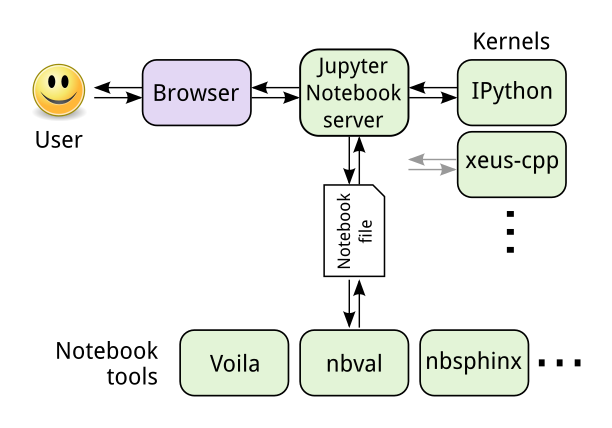
\includegraphics[width=0.6\textwidth]{images/notebook_components.png}
  \caption{The architecture of the Jupyter Notebook, kernels, and tools
        which operate on notebook files}
  \label{fig:notebook-architecture}
\end{figure}

\medskip
\noindent\textbf{Related projects}

EOSC-hub is a 33 million Euro H2020 project that started in January 2018 with
the involvement of over 100 institutes. In three years the project is
establishing the first elements of the European Open Science Cloud. EOSC-hub
defines, creates and operates the integration and management system of the
EOSC.  This integration and management system (the Hub) builds on mature
processes, policies and tools from the leading European e-infrastructures to
cover the whole life-cycle of services from planning to delivery. Through this
management system online and `human' services, software and data are delivered
towards researchers via a single EOSC Portal. The Marketplace already includes
nearly 50 services from EOSC-hub provided by 3 e-infrastructure communities
(EGI, EUDAT, INDIGO-DataCloud), and from 18 Research Infrastructures and
scientific service providers. The catalogue of services is expected to
radically grow in the next years through national, regional and EU
initiatives.

Integrating Jupyter-based services into EOSC provides an excellent opportunity
for facilitating interoperability of EOSC services,
bringing data and computation together in a flexible environment.

\subsubsection{Methodology}\label{sec:methodology}


\textbf{Proposed improvements to core components of Jupyter (\WPref{core})}\\
We plan to make technical changes to Jupyter software to better support
real-time collaboration (\taskref{core}{collaboration}),
so that two or more people in different places or working on different
devices can work together
on the same notebook. This would significantly enhance the value of
notebooks for collaborative research.
We will also work on making Jupyter software accessible to as broad a
range of users as possible (\taskref{core}{accessibility}).

Further work to bring the code behind JupyterHub and Binder closer together
(\taskref{core}{jh-bh-conv}) will bring a range of benefits, allowing more
flexible sharing of notebooks along with access to remote computing resources
such as those available through EOSC.

Finally, we are explicitly allocating time in \WPref{core} for maintaining
Jupyter software, as well as new development (\taskref{core}{maintenance}).
Maintenance is crucial to creating reliable, sustainable software,
but its cost is often swept under the rug in funding applications
because of the perceived pressure to focus on novelty.
Being up front and explicit about this cost is critical to the sustainability
of open source open science.

\medskip
\noindent\textbf{Proposed improvements to the Jupyter ecosystem (\WPref{ecosystem})}\\
We further propose improvements to the wider Jupyter ecosystem for
better scientific workflows. In particular, we have identified
possible improvements to:

\begin{itemize}
  \item Binder and its crucial software component \emph{repo2docker}
    (\taskref{ecosystem}{r2d-and-binder}).

  \item Xeus, to better support the C++ programming language in notebooks
    (\taskref{ecosystem}{xeus-cpp}).

  \item Interactive widgets, including tools for 3D visualisation to help
    people make sense of large amounts of data
    (\taskref{ecosystem}{jupyter-widgets}).

  \item Archiving of computational environments to allow reproducible research
    with a focus on the long term (\taskref{ecosystem}{reproducibility}).

  \item Tooling and guidelines
    for using notebooks in education
    (\taskref{ecosystem}{teaching-tools}).

\end{itemize}

We may create new open source software projects in these tasks,
but we will carefully review existing software, both in the
Jupyter ecosystem and beyond, to avoid unnecessary duplication of effort.

\medskip\noindent\textbf{Beyond the improvement to the Jupyter Project
  (\WPref{applications}, \WPref{eosc}, \WPref{education})}\\
Beyond the improvement to the Jupyter core and ecosystem software for EOSC, we plan on
\begin{itemize}
\item Design, implementation, application, demonstration and
  evaluation of new innovative EOSC services
  in multiple demonstrators, that cover research fields such as
  health, astrophysics, photon and neutron science, geosciences and
  mathematics, and also interests of participating SMEs (\WPref{applications}).
\item Operating a \emph{European Binder Service} on the EOSC-Hub and
  enabling provision of Jupyter Services through the EOSC-Hub (\WPref{eosc}).
\item Producing \emph{training and education material} to disseminate
  the ability to do reproducible computational science using the tools
  we develop, among others (\WPref{education}).
\end{itemize}

\medskip
\noindent
\textbf{The science
  demonstrators}\label{sec:science-demonstrators-in-concept}\\

We describe the context and challenges for each demonstrater in this
section. The particular planned activities are shown in the
corresponding tasks in \WPref{applications}.\\

\noindent\textbf{Demonstrator: Astronomy (\taskref{applications}{astro})}\label{sec:concept-demonstrator-astronomy}\\
  The \href{http://cdsweb.u-strasbg.fr/}{Strasbourg Astronomical Data Center} (CDS) is a scientific data
  center hosted by the Observatory of Strasbourg. The CDS plays a unique and
  essential role in astronomy by adding value to published and reference data.
  CDS runs astronomical services that
  provide data for the world-wide astronomy research community. Its three main
  services (SIMBAD, VizieR and Aladin) are heavily used with up to one million
  queries per day.  These services can be accessed through web interfaces, mainly
  for human interaction, as well as through programmatic interfaces, including
  the standardized protocols defined by the International Virtual Observatory
  Alliance \cite{ivoa}.

\begin{figure}[ht!]\centering
  \includegraphics[width=0.6\textwidth]{python-astro-citations}
  \caption{Mentions of programming languages in refereed Astronomy papers, extracted from ADS. Python usage has increased dramatically in the recent years.}\label{fig:python-astro-citations}
\end{figure}

  Python and notebooks are rapidly increasing in importance for astronomy
  research. Indeed, Python for Astronomy software ecosystem has known a
  constant steady growth in the latest years, as shown in
  figure~\ref{fig:python-astro-citations}. As Python and notebooks integrate
  well together, the Jupyter notebook as an analysis tool is becoming a hot
  topic in the astronomical world: large surveys like the LSST (Large Synoptic
  Survey Telescope) have endorsed the usage of the Jupyter platform for their
    data access portal \cite{lsst2017scienceplatform}.\\


  We will develop a Jupyter-based framework to efficiently access, explore,
  visualize and analyze reference data that are available through CDS services
  as a real example of using open astronomy data.
  We will provide scientific users with a set of customizable Jupyter notebooks
  for visualization and analysis tasks, providing a new level of
  interoperability with python libraries and notebooks as is highly demanded
  by the astronomy research community.

  The focus is on the two following user stories:
    \begin{compactitem}
        \item analysis of catalogue data results, up to billions of rows.
              Tabular data is the typical output of SIMBAD and VizieR data.
        \item modular dashboard-like interface providing a top level
              interactive view of the available data for a given astronomical
              object and enabling loading and analysis of those data.
    \end{compactitem}


\begin{figure}[ht!]\centering
  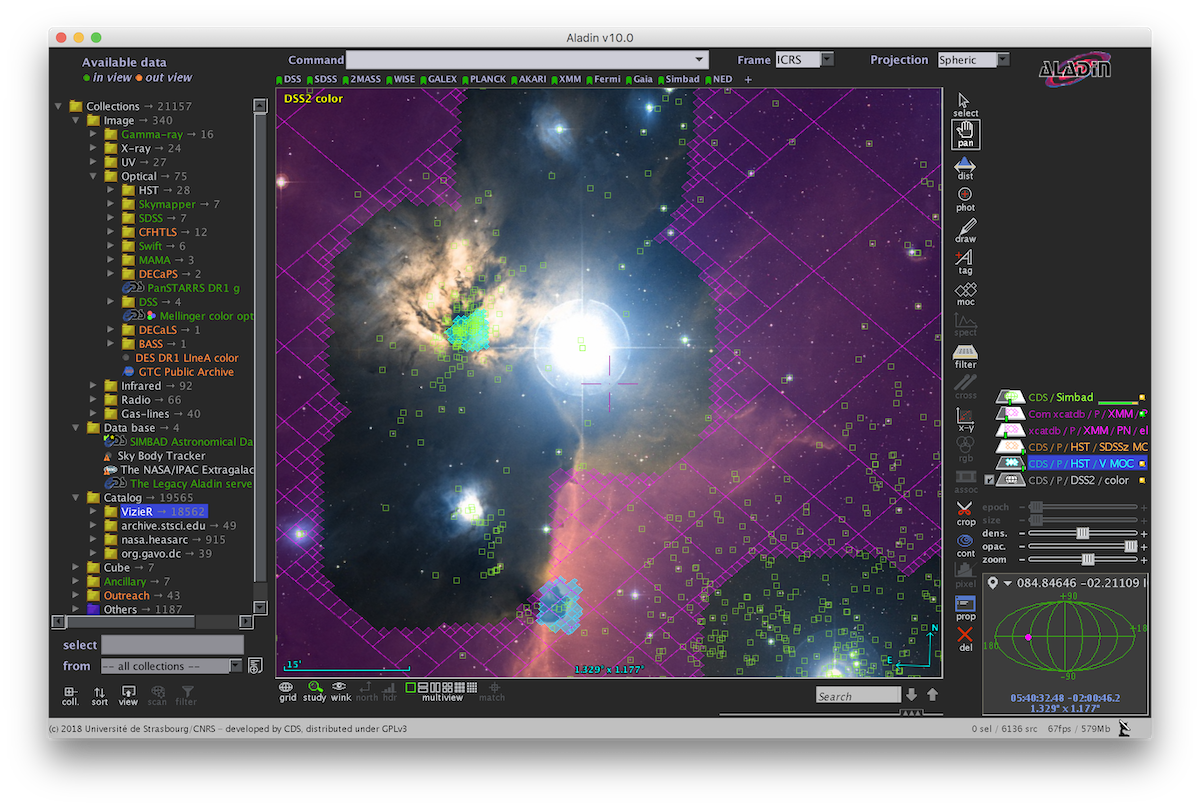
\includegraphics[width=1.0\textwidth]{astro-aladin-snapshot}
  \caption{Example of astronomical data objects: Simbad sources, XMM and Hubble coverages overlaid on Digital Sky Survey imagery in the vicinity of the Horsehead nebula, and visualized in Aladin Desktop software.}\label{fig:astro-aladin-snapshot}
\end{figure}

  Access to the notebooks will be provided as a one-click action option from
  SIMBAD and VizieR results pages.
  Thus, providing with a one-click way of visualizing, filtering and analyzing
these potentially large tables will bridge the gap between access and analysis
of the data, with zero installation for the user.
  For specific science cases, we will explore rendering of notebooks with
  interactive widgets through Voila \cite{Voila}, as to allow users not familiar with
  Python to benefit from the Jupyter notebook framework.
  Figure~\ref{fig:astro-aladin-snapshot} depicts typical data objects we want to analyse and interact with in the notebooks: images, catalogue data, datasets coverages.

  These new developments will be highly visible to the large number of astronomers who use the CDS services (50,000 unique visitors per month) and such tools are in high demand by these users.

  The CDS expertise in astronomy data and interfaces will be profitably combined with expertise of BOSSEE partners to ensure the deployment of high quality widgets (Simula, WildTree Tech, QuantStack).

  The particular activities for this demonstrator are shown in
  \WPref{applications} in \taskref{applications}{astro}.

\medskip
\noindent\textbf{Demonstrator: Enriched education with Jupyter (\taskref{applications}{teaching})}\label{sec:concept-demonstrator-teaching}

  In the recent years, Jupyter technologies have been widely adopted
  worldwide in higher education -- and even in high schools -- for
  teaching in all areas of sciences. The Jupyter notebook indeed
  provides a very versatile environment -- with a smooth learning
  curve -- for authoring interactive material such as class notes,
  exercise sheets, dedicated applets; all the way to complete books
  such as those produced by OpenDreamKit for biology, physics, and
  mathematics. The interactivity engages the students to take an
  active role, for example playing with code, exploring the effect of
  tweaking the parameters in a simulation, changing visualizing tools,
  adding personal notes. This lets them take progressively ownership
  of the material and better understands the issues, and encourages
  them to create their own documents and share their experience with
  colleagues and teachers.

  \begin{figure}[ht!]\centering
  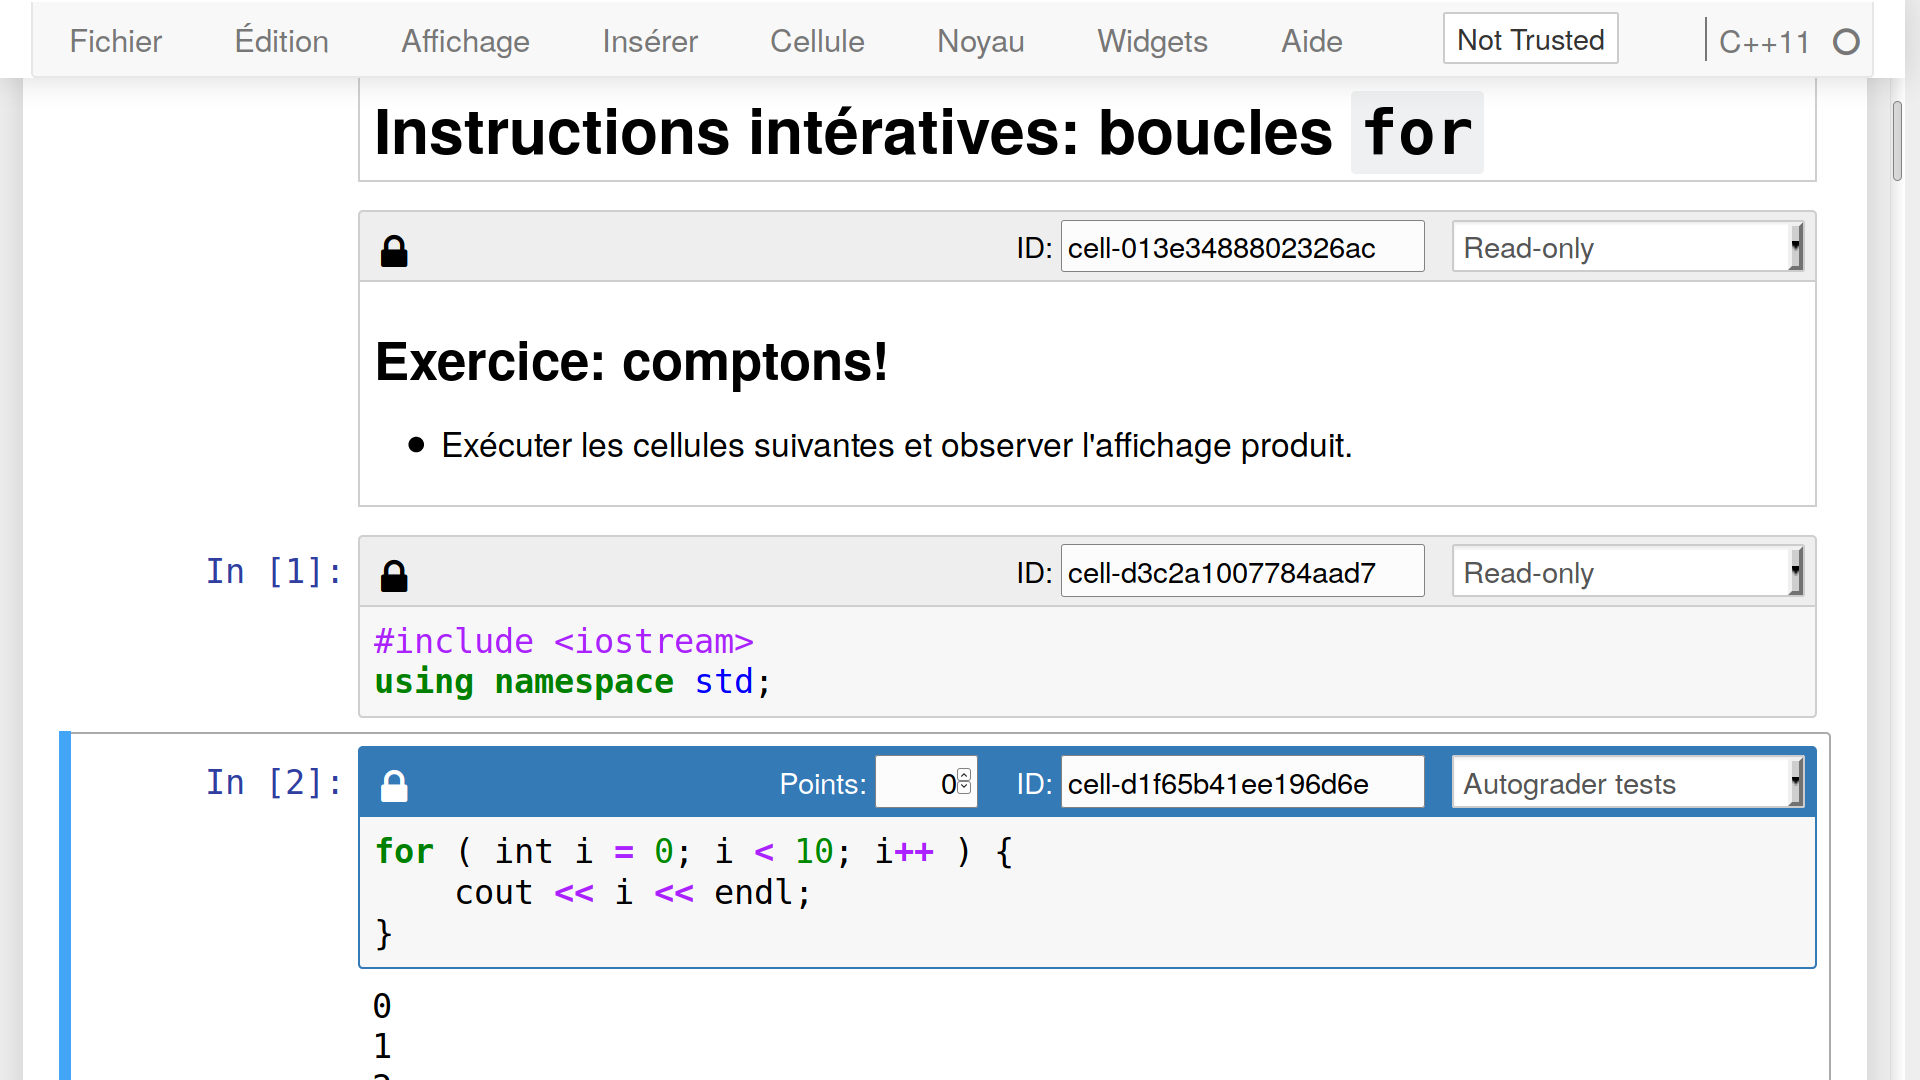
\includegraphics[width=.45\textwidth]{images/teaching-cling}\quad
  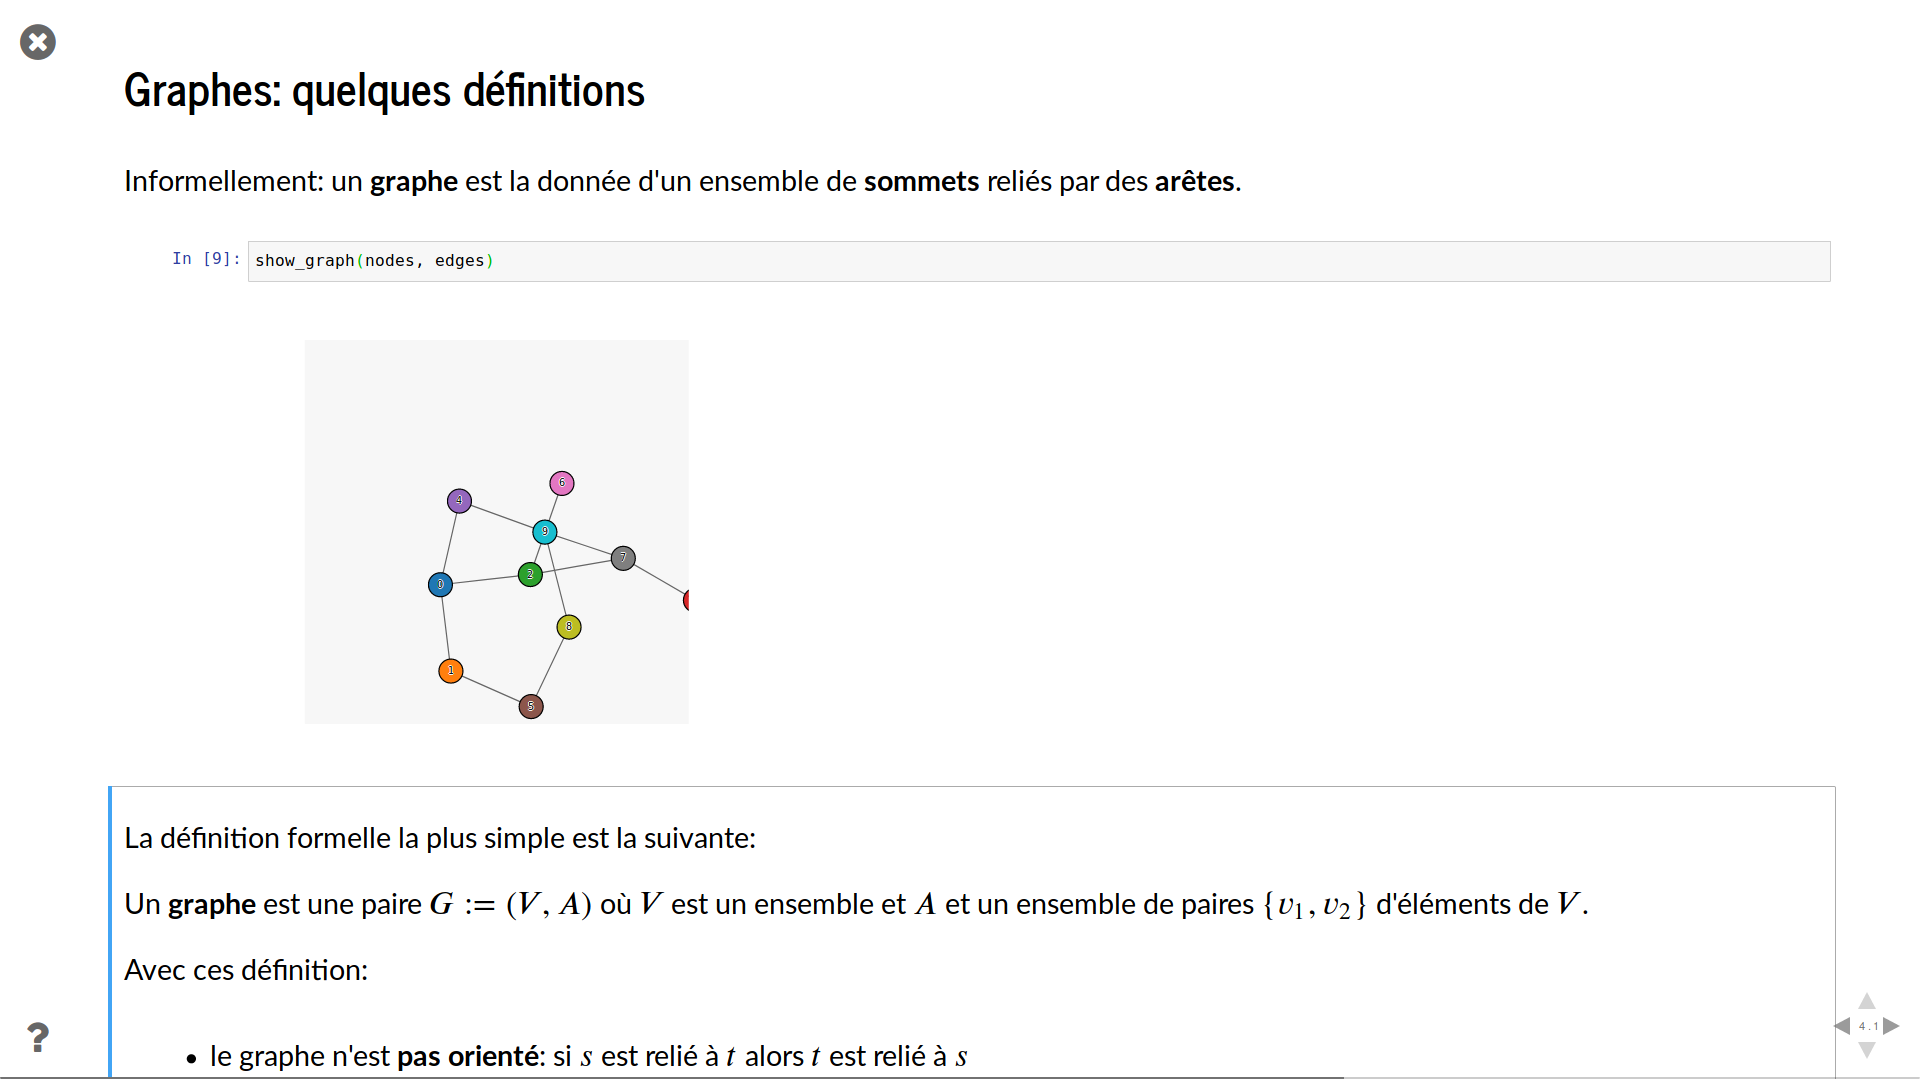
\includegraphics[width=.45\textwidth]{images/teaching-graphs}
  \caption{Jupyter based teaching material from Paris Sud. On the
    left: an exercise sheet for the course \emph{Introduction to
      programming}; this instructor version showcases interactive C++
    execution and automatic grading configuration menus. On the right:
    interactive slides for a graph theory course.}\label{fig:teaching-cling}
  \end{figure}

  Success stories include:
  \begin{itemize}
  \item Berkeley's ``Data 8: The foundations of Data Science'' open
    course (\url{data8.org}) which is delivered yearly to thousands of
    lower undergraduate students in all majors, scientific or not,
  %\item OpenAI Gym (\url{https://gym.openai.com/}), 
  \item QuantEcon' open interactive book ``Lectures in Quantitative
    Economics'' (\url{https://lectures.quantecon.org/}), entirely
    authored with Jupyter.
  \item 100+ IPython/Jupyter based MOOC's (Massively Open Online
    Courses) on Coursera
    (\url{https://www.coursera.org/courses?query=ipython})
  \item Paris Sud's first-year course ``Info 111: Introduction to
    Computer Science'' where each year 400 students write their first
    lines of code in C++ in a Jupyter notebook (see Figure~\ref{fig:teaching-cling}).
  \end{itemize}

  École Polytechnique, Université Paris-Sud, and other participants from this
  project have been early adopters of these tools (see the description of \site{EP}
  and \site{UPSUD}, and also task~\taskref{ecosystem}{teaching-tools}).
  We learned the hard way that deploying the Jupyter environment at a
  large scale (e.g. for a university) requires specialized expertise
  (DevOps, software development, ...) which impedes its adoption
  by the greatest number of people. High quality hosted solutions
  (e.g. CoCalc\cite{Cocalc}, Gryd\cite{Gryd}) do exist but are not the final solution when it
  is desired to exert greater control on private data, integration with
  the local infrastructure (authentication, shared drive, e-learning
  environment, dedicated hardware, ...), or to use available local computing
  resources rather than paid services.

  Further improving the Jupyter environment for education, while
  leveraging it to the greatest degree, are therefore key motivations
  for the following tasks of this proposal:
  \begin{itemize}
  \item Tasks~\taskref{core}{jh-bh-conv}
    and~\taskref{eosc}{jh-bh-deployment} will greatly ease the
    deployment of Jupyter environments, with tight integration in the
    existing local infrastructure and full customizability by the
    teachers.
  \item Task~\taskref{ecosystem}{teaching-tools} will improve the
    interoperability with existing e-learning systems, and further
    develop teaching aids for, e.g., material sharing,
    (self)-evaluation, and grade management.
  \item Task~\taskref{applications}{math} will support teaching
    in mathematics through better support for real-time interactivity.
  \item Task~\taskref{ecosystem}{xeus-cpp} will support teaching
    in computer-science and scientific programming through
    better C++ integration in the notebook and will allow to first class students to focus on the
    syntax of the language without distractions such as compiling and
    linking a program.
  \item Task~\taskref{eosc}{eosc} will ease publication and FAIR
    access to course material, which in turn will promote sharing
    and collaboration in the education community.
  \end{itemize}

  The particular activities for this demonstrator are shown in
  \WPref{applications} in \taskref{applications}{teaching}.

\medskip
\noindent\textbf{Demonstrator: Visualisation and control of fluid dynamics in
  Jupyter notebook (\taskref{applications}{application-gpu})}\label{sec:concept-demonstrator-gpu}\\
In recent years, the lattice Boltzmann method (LBM) emerged as an
interesting alternative to more established methods for fluid flow
simulations. Sailfish-cfd \cite{januszewski2014sailfish} is an open
source implementation of the LBM on General Purpose Graphical Processing
Unit (GPGPU) devices. It is written in Python with real-time
generation of CUDA-C code.  In order to harvest capabilities of GPGPUs
one needs to access the specialized hardware, which usually is
available to researchers as remote HPC resources.  The typical fluid
dynamics research workflow consists of three stages: preparing
boundary conditions, running a simulation, and data analysis. The
first and last stage require capable and responsive user interface for
maniputation and inspection of 3d data.  The Jupyter 3d visualisation
widgets developed in \taskref{ecosystem}{jupyter-widgets} can fulfil
such needs.

Based on previous experience with K3D-jupyter~\cite{K3D}
widgets we know that web browser based software can display moderate
dataset during the simulation. As the dataset is becoming larger the
visualisation in the browser turns out to be nontrivial due to
limitations of the browser itself and required large data transfers. It is
an open question how much of data processing should be performed on
server-side and what can be done on the client hardware (i.e. in the
widget in the browser side of the user). Our
experience suggests that there is no clear answer and it depends on
the size of the data and its nature. For example, volume rendering
technique can be very effective on the browser side but infers large data
transfers. One can perform it the server-side, in a distributed way if
the simulation uses many nodes, but the interactivity is limited by
network latency. We will attempt to provide practical
solutions to this issue.
%
  \begin{figure}[ht!]\centering
  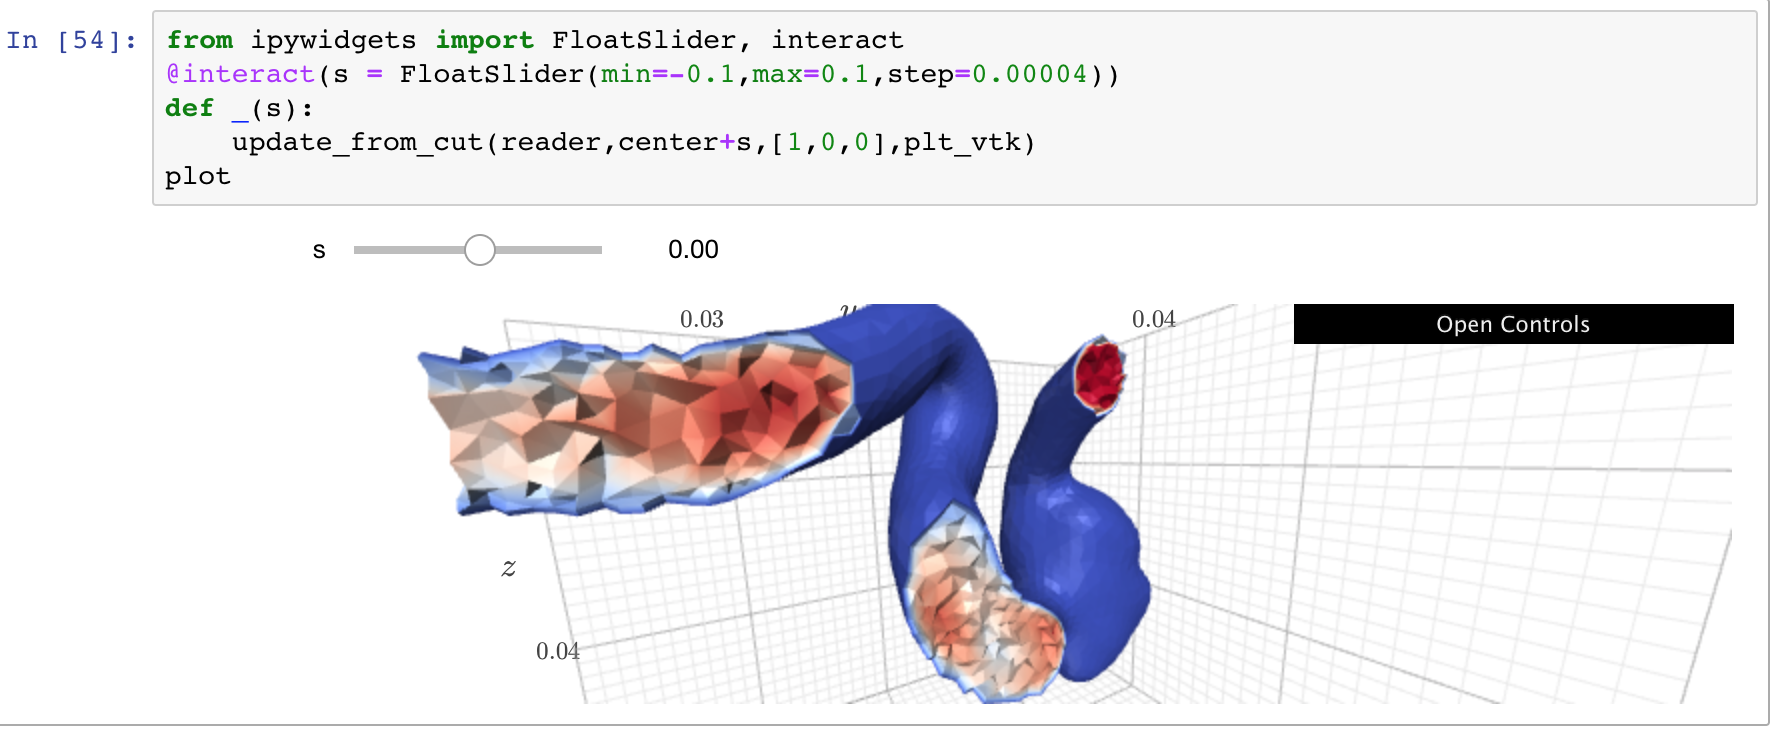
\includegraphics[width=.95\textwidth]{images/k3d_cfd.png}
  \caption{An example showing Jupyter based visualization of velocity
    magnitude in the blood flow through an aneurysm. It demonstrates
    the use of small interactive widget for selecting the cutting
    plane.
    Visualization is done by a K3D-jupyter widget~\cite{K3D}.
    In this case most of computations are done using VTK library on
    the server side, and the K3D-jupyter widget is used to display the
    colored surface mesh.
  }\label{fig:k3d-cfd}
  \end{figure}

    The particular activities for this demonstrator are shown in
  \WPref{applications} in \taskref{applications}{application-gpu}.

\medskip
\noindent\textbf{Demonstrator: Geosciences (\taskref{applications}{geoscience})}\label{sec:concept-demonstrators-geo}\\
The amount of geospatial data from a variety of sources, including satellite observations, 4D simulations and in-situ observations, contributed by volunteers
or state agencies keeps increasing. In many disciplines, managing this large volume
has become a challenge, and the old approach of downloading datasets for local
analysis has become intractable.

The heterogeneity of the tools used in different institutions to deal with
large geographical datasets makes it difficult for researchers to share the outcome
of their work in a reproducible or interoperable fashion.

In this context, Jupyter is now emerging as a standard exploration tool for
geospatial analysis, climate science, geology and by data providers in these areas.

To mention a few,
\begin{itemize}
\item
   the \emph{PanGeo} platform \cite{Pangeo2018} (Funded by the NSF, NASA, and the
   Alfred P. Sloan Foundation) is built upon Jupyter, JupyterHub, Binder, and Dask.
\item
   the \emph{Joint Research Centre Earth Observation Data and Processing Platform}
   (JEODPP) \cite{Soille2018} relies on Jupyter, JupyterHub and ipyleaflet as
   its main user interface (see also figure~\ref{fig:jeodpp} on page \pageref{fig:jeodpp}).
\item
   the \emph{Google Earth Engine} platform also offers a Jupyter-based user
   interface allowing the visual exploration of the data with ipyleaflet
   \cite{GEEJupyterLeaflet2017}.
\end{itemize}

In these three cases, deferred processing is used to restrict computation to
the extent of the area displayed in the map viewer, which allowed these
platforms to scale up to petabytes of data. In all examples, interactive
visualization is a key feature of the platform. Beyond tile-based
2-D visualization, the ability to efficiently process and visualize vector
or 3-D  data is also becoming critical.

The BOSSEE team, which comprises the main authors of the technologies upon
which these platforms are built (Jupyter, JupyterHub, Binder, ipyleaflet),
together with the Department of Geosciences of the University of Oslo, are
in a unique position to bring these technologies together in the context of
EOSC.

This demonstrator will focus on tools for two transversal research projects

\begin{itemize}
\item \href{https://www.mn.uio.no/geo/english/research/groups/latice/}{LATICE} (Land-Atmosphere Interactions in Cold Environments)
\item \href{https://www.mn.uio.no/geo/english/research/groups/earthflows/}{EarthFlows} (Interface Dynamics in Geophysical Flows)
\end{itemize}

The work items for this demonstrator fall in two main categories:
visualization and geographical data processing tools. Data will not be produced as part of \TheProject. The University of Oslo follows the "open as standard" policy and all data used for \TheProject will be publicly available through:
\begin{itemize}
\item the \href{https://archive.norstore.no/}{Norwegian Research Data archive}
\item \href{https://zenodo.org/}{Zenodo} for smaller datasets and for datasets used for teaching
\item SQL requests for in-situ observations stored in local databases (for instance collected during field campaigns)
\item the Earth System Grid Federation (ESGF) for all climate data,
\item \href{https://www.copernicus.eu/en/access-data}{Copernicus data portal} for satellite observations.
\end{itemize}


Beyond their use in scientific research, these development will be used in
the class room for teaching master's students with best practices in open
science.

The particular activities for this demonstrator are shown in
  \WPref{applications} in \taskref{applications}{geoscience}.

\medskip
\noindent\textbf{Demonstrator: Nuclear Medicine dosimetry (\taskref{applications}{opendose-analysis})}\label{sec:concept-demonstrators-opendose}\\
  % Scientific description
  Nuclear Medicine is a field of medicine where radioactive material
  (radiopharmaceutical) is used for diagnostic and therapy. The OpenDose
  project \cite{Chauvin2017} is a collaborative effort to generate a reference
  database, freely available, proposing dosimetric data applicable in a context
  of nuclear medicine dosimetry.  A major aspect of the project is the
  development of tools ensuring traceability and reproducibility of generated
  results.

  \begin{figure}[ht]
    \centering
    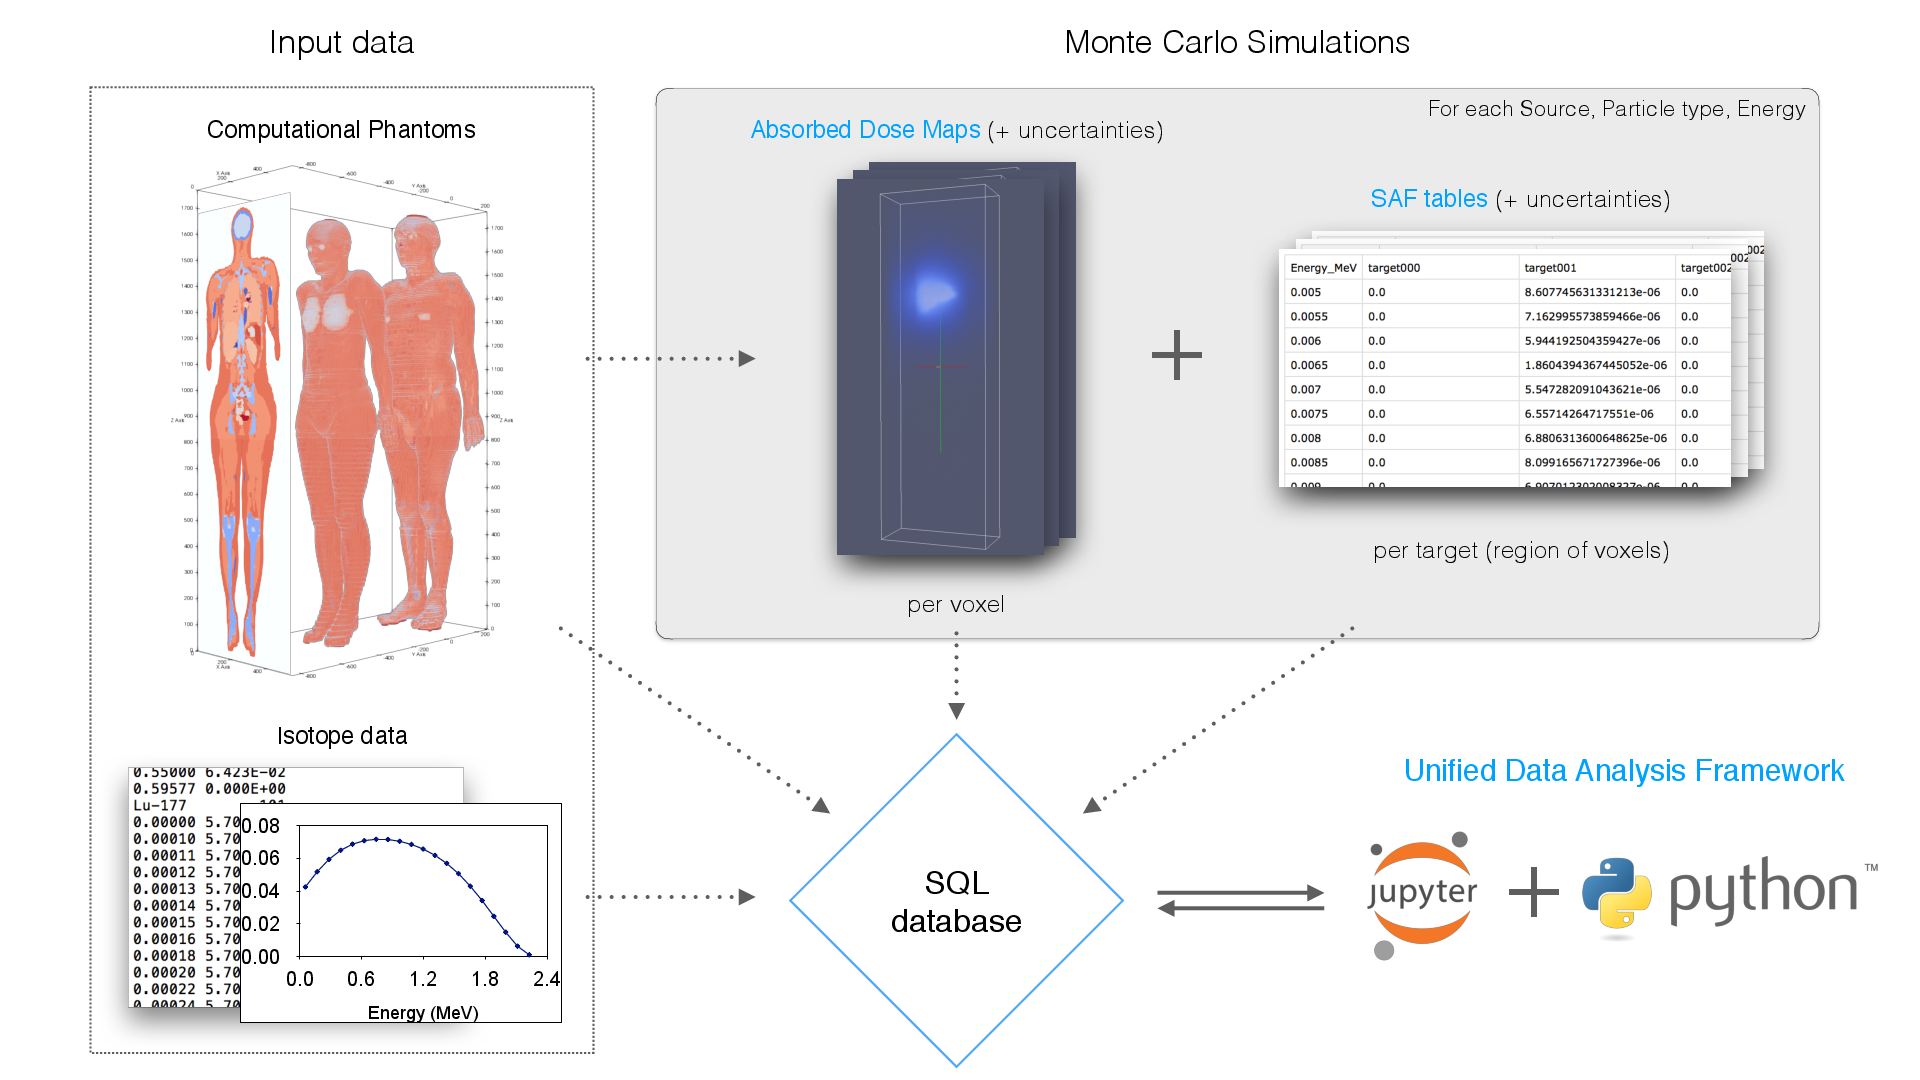
\includegraphics[width=1.0\textwidth]{images/opendose_framework.png}
    \caption{OpenDose project overall framework including the unified data
    analysis to be developed in this demonstrator.}
    \label{fig:opendose_framework}
  \end{figure}

  % Technical description
  OpenDose data is produced using the five most represented Monte Carlo
  simulation software tools in medical applications: Geant4/GATE, MCNP, EGS, PENELOPE
  and Fluka. Each simulation consists of calculating radiation transport in
  anthropomorphic models for specific parameters (source organ, particle type,
  energy, model and number of primaries to simulate). Every simulation produces
  binary (3D matrices) and ASCII files for a total of $\sim$150MB / simulation.
  The 3D matrices contain energy deposited per voxels, and ASCII files contain
  pre-processed data corresponding to energy deposited per regions such as
  organs and tissues. These raw outputs are later processed into dosimetric
  data such as Specific Absorbed Fractions (SAFs) and S-values.

  Producing data for one model (ex. Adult female) requires $\sim$30,000
  simulations, with the workload shared between the different teams and
  software.

  The data produced by all the teams is currently centralised at the Cancer
  Research Center of Toulouse (CRCT), processed and fed into a local SQL
  database at CRCT.

  This collaborative effort raises some challenges:
  \begin{compactitem}
  \item Data production: a total of 750,000 hours of CPU time is needed per
    model.
  \item Volume of data: one model represents TBs of raw data that can be
    heterogeneous from the different teams.
  \item Data analysis: raw data has to be processed into dosimetric data in a
    robust and reproducible way.
  \item Database: has to be efficient and handle all the data (raw and
    processed).
  \item Visualization: display and compare results from all teams.
  \end{compactitem}

  Figure \ref{fig:opendose_framework} shows the overall framework of the
  project and how data will be managed.

  By building a set of tools to access and process data within the Jupyter
  ecosystem, we will ensure the production of traceable and reproducible
  dosimetric data for the OpenDose project members.

  Another major aspect of the OpenDose collaboration is to provide open
  access to the generated dosimetric data. For that purpose a website is under
  development to allow data download and simple dosimetry calculations. For
  users who need more advanced calculations, a dedicated Jupyter workspace will
  provide a set of tools to easily access, process and display the OpenDose
  data.

  The particular activities for this demonstrator are shown in
  \WPref{applications} in \taskref{applications}{opendose-analysis}.

\medskip
\noindent\textbf{Demonstrator: Interactive Mathematics with Jupyter Widgets (\taskref{applications}{math})}\label{sec:concept-demonstrator-math}\\
  Computations have played a long time and ever increasing role for
  research and teaching in (pure) mathematics, to explore, search and
  check for conjectures, or better understand algorithmic ideas. This
  led to the development of a whole ecosystem of mathematical
  software, many of which are open source. Given the huge variety of
  mathematical objects and workflows, the Read-Eval-Print-Loop (REPL)
  paradigm -- on which Jupyter is based -- is particularly suitable:
  the user interacts with the system by typing commands that use its
  library of mathematical features, often combined with personal code.
  In fact, the REPL and notebook paradigms of Jupyter as well as some
  of its interactive features were largely inspired by that of
  computer algebra systems such as Maple, Mathematica, or SageMath.

  One major action of the OpenDreamKit project was to foster the
  convergence between the Jupyter and math software ecosystems:
  nowadays Jupyter can be used as a uniform user interface for most
  major systems: e.g. GAP, OSCAR, Pari/GP, SageMath, Singular, and
  even for C++ libraries. This interface is being widely adopted: for
  example, Jupyter has become the standard user interface for
  SageMath, enabling to phase out its former bespoke notebook; by now,
  thousands of Jupyter notebooks for SageMath are publicly shared
  (6000+ on GitHub alone).

  Thanks to this prior work, the mathematical community will
  immediately enjoy all the benefits brought by EOSC-based generic
  Jupyter services, including eased collaboration, sharing, archival,
  and reproducibility.

\begin{figure}[h]
  \begin{center}
    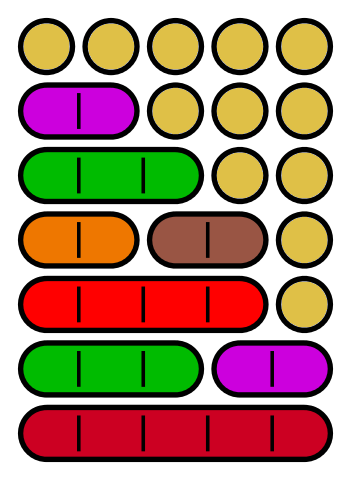
\includegraphics[height=2.9cm]{images/partitions-of-5}
    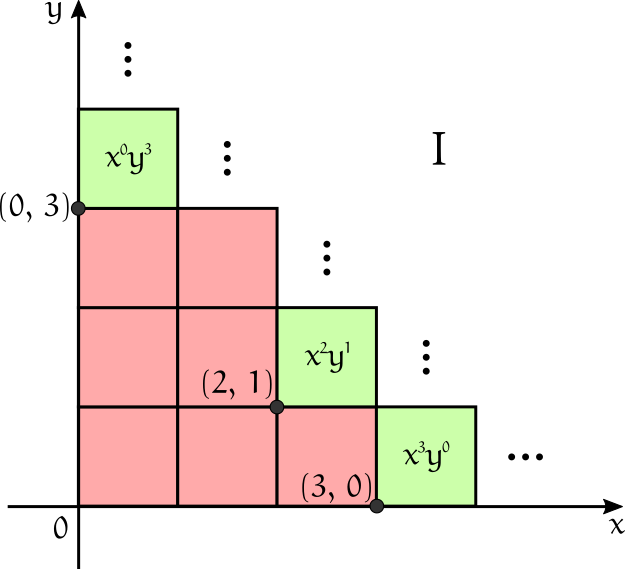
\includegraphics[height=2.9cm]{images/Wikipic}
    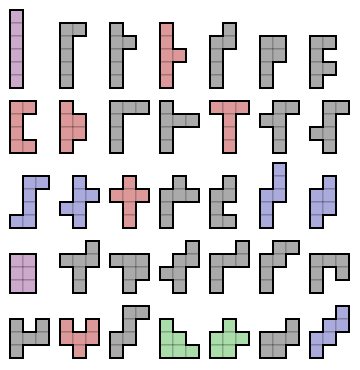
\includegraphics[height=2.9cm]{images/hexominoes}
    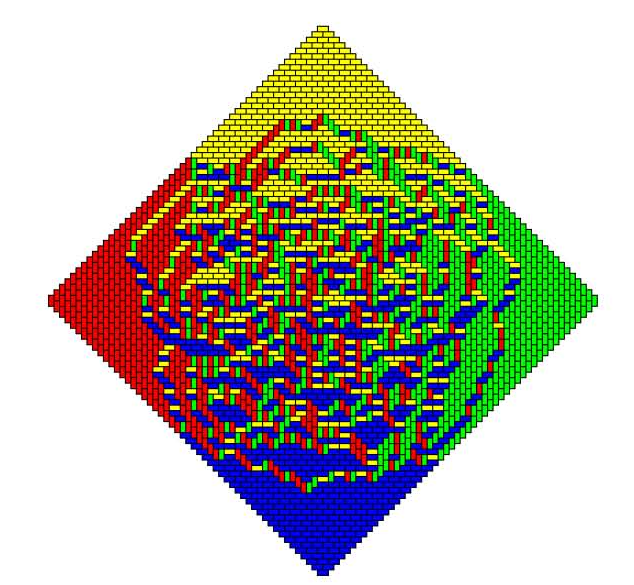
\includegraphics[height=2.9cm]{images/AztecDiamond}
    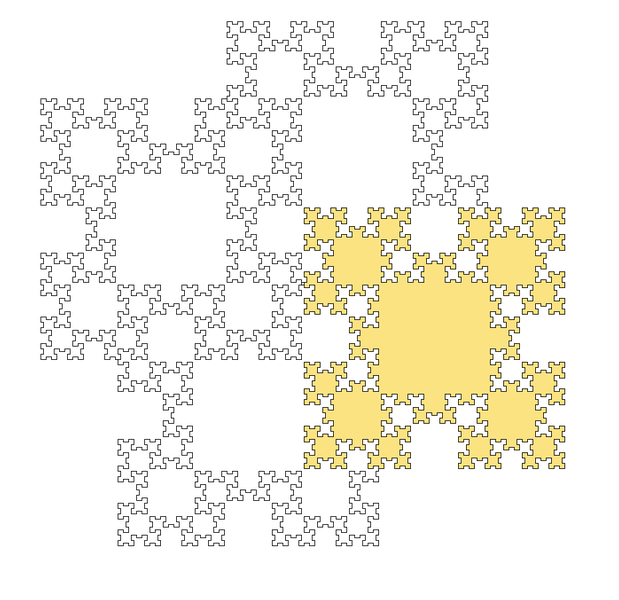
\includegraphics[height=2.9cm]{images/619px-Tiling_Fibonacci_word_fractal}
    \medskip

    
\includegraphics[height=2.5cm]{images/fractioncont}
    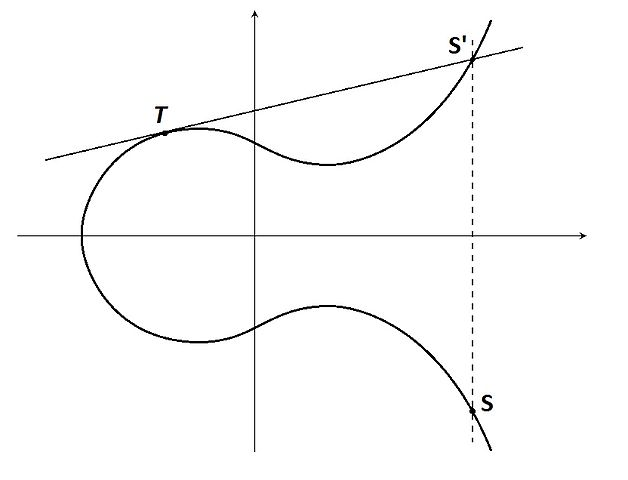
\includegraphics[height=2.9cm]{images/elliptic-curve}
    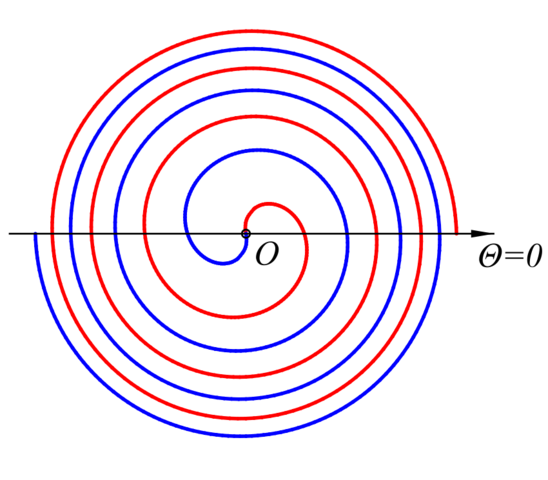
\includegraphics[height=2.9cm]{images/548px-Fermat's_spiral_01}
    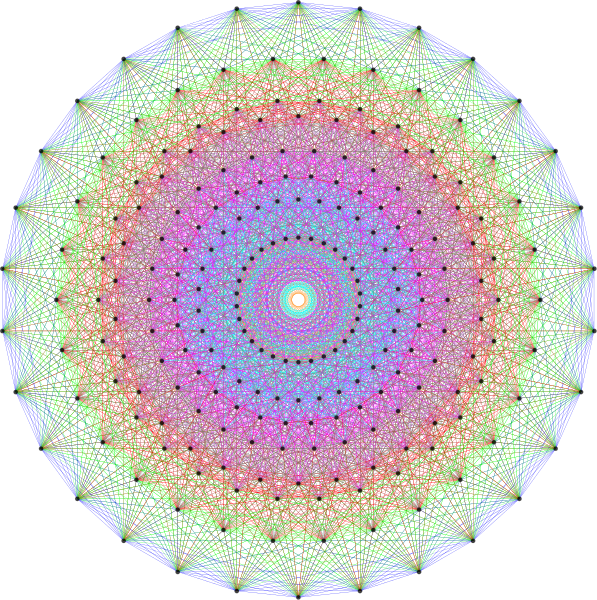
\includegraphics[height=2.9cm]{images/597px-E8Petrie}
    \medskip

    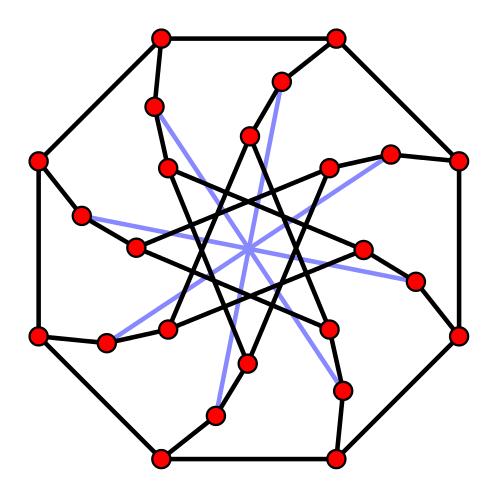
\includegraphics[height=2.9cm]{images/500px-McGee_graph}
    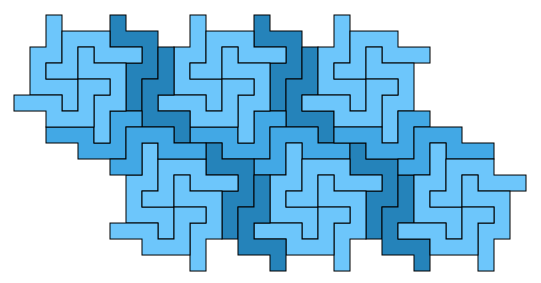
\includegraphics[height=2.9cm]{images/nonominoes}
    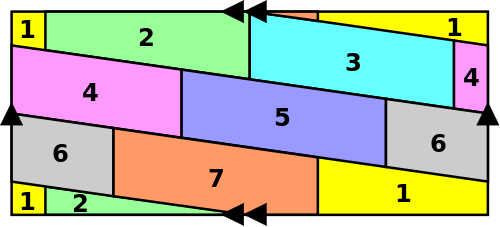
\includegraphics[height=2.9cm]{images/500px-Torus_with_seven_colours}
    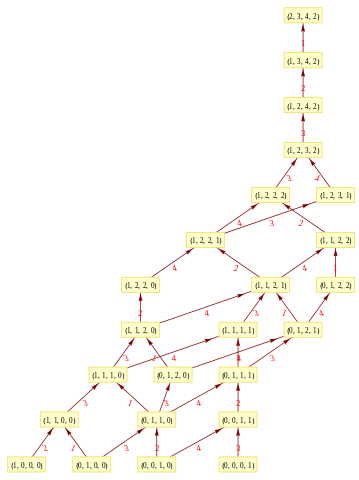
\includegraphics[height=2.9cm]{images/359px-F4HassePoset}
  \end{center}
  \caption{Graphical visualizations of a variety of mathematical objects}
  \label{fig:math_viz}
\end{figure}

  The next step to maximise attractivity and impact in the
  mathematical community, and this is the aim of this task, is to go
  beyond the REPL paradigm, and \textbf{leverage the real time
    interactivity and flexibility brought by Jupyter widgets for
    Mathematical purposes}. This will, for example, make it straightforward for a teacher or
  researcher to build and disseminate via the EOSC mini applications
  or dashboards enabling the graphical exploration of a whole range of
  mathematical inputs, with real-time visualization of the associated
  outputs.

  The unique challenge comes from the huge variety of mathematical
  objects that the user may want to visualize and interact with, and
  the variety of graphical representations (see Figure~\ref{fig:math_viz}). Co-design is central here,
  as building a bespoke interactive visualization entails a
  combination of technology skills (e.g. javascript development) and
  business knowledge (designing the interaction and visualization).
  The role of Research Software Engineers is to leverage the
  technology by encapsulating the technical difficulties into flexible
  and easy to use tool boxes from which mathematicians can build
  mini-applications as innovative services that are tailored to their needs.

  Within OpenDreamKit, we conducted experiments to explore this
  venue~\cite{ODK_D4.16}. One specific focus was to enable not only
  \emph{interactive visualization}, but also \emph{interactive
    editing}: being able to graphically modify the mathematical object
  being visualized; this enables the interactive exploration of how the
  modifications affect its properties, or to use the editor as an input
  widget for a larger application or dashboard. The outcome of this
  task is the development of two prototypes in SageMath
  (\software{sage-combinat-widget}, a library of widgets for
  combinatorics, and \software{sage-explorer} a generic dashboard for
  interactive browsing and introspection of mathematical objects), and
  contributions to \software{Francy}, an Interactive Discrete Math
  Framework for \software{GAP} and \software{SageMath}.
  \TODO{... which are accessible as an EOSC service?}

  The particular activities for this demonstrator are shown in
  \WPref{applications} in \taskref{applications}{math}.

\medskip
\noindent\textbf{Demonstrator: Reproducible photon science workflows at
  European XFEL (\taskref{applications}{reproducibility-xfel})}\label{sec:concept-demonstrator-photonscience}\\


  European XFEL is a research facility that provides X-ray Free
  Electron Laser (XFEL) light to image structures at the nanoscale. It
  is currently the world's most brilliant laser, created in a 3.4km
  long tunnel, and supporting user experiments since September
  2017. These imaging capabilities of European XFEL and similar
  services available from synchrotron and neutron sources, underpin lots of
  fundamental and applied research, in domains ranging from
  physics and material science to biochemistry and drug design. Some
  example data is shown in figure \ref{fig:photon-science-example}.

  All of the data recorded at European XFEL will be made freely
  available after an embargo period of three years
  \cite{EuXFEL-datapolicy-2017}. This provides scientific transparency
  and is expected to enable better exploitation of the data, as more
  researchers than those conducting the experiments have access to the
  results. If the analysis steps are not carefully recorded, there is a risk
  that the necessary understanding of the data is lost by the time it
  is made public or subsequently, greatly reducing its scientific
  value.

  We are keen to complement this open data access to the actual data
  with open access to reproducible data analysis, to confirm
  conclusions drawn and to significantly lower the barriers for
  re-analysis with new tools or for new research purposes.

  A task in the EC funded project Photon and Neutron Open Science
  Cloud (PaNOSC) is using the Jupyter Ecosystem tools as they are in
  2019 to provide interactive data analysis services to complement the
  data: through use of Jupyter Notebook and exploitation of the
  mybinder.org service, this activity will reduce the barrier for
  interactively exploring the data, understanding and making use of
  the data, and to do this through a central portal such as EOSC.

  Here, we combine and use the new developments (\WPref{core},
  \WPref{ecosystem}) of this
  proposal to enable new qualities of open science services, and to
  demonstrate the potential impact of these improvements for a wide
  set of EOSC services through a demonstrator in Photon Science.

  \medskip

\begin{figure}[tb]
    \centering
    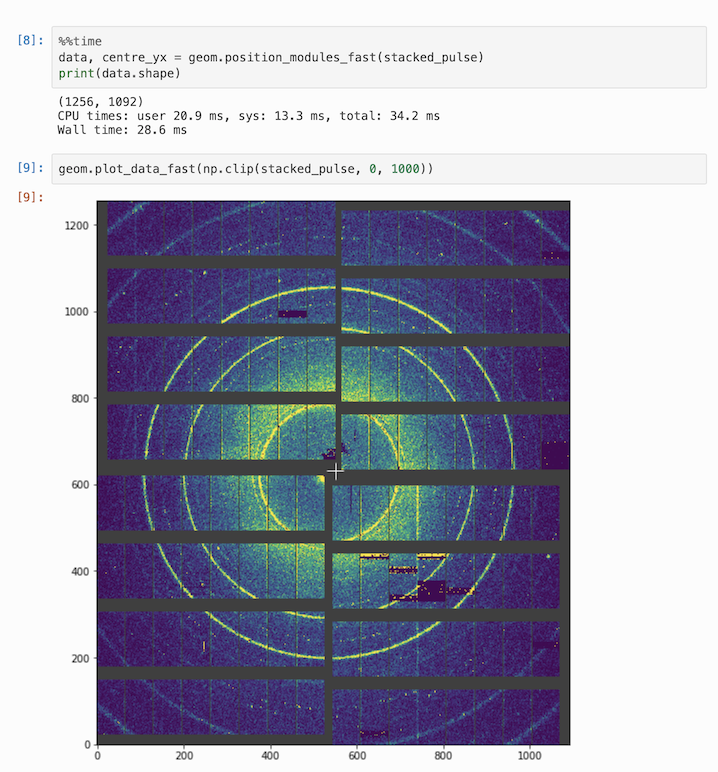
\includegraphics[height=0.27\textheight]{images/photon-science-prototype1.png}
    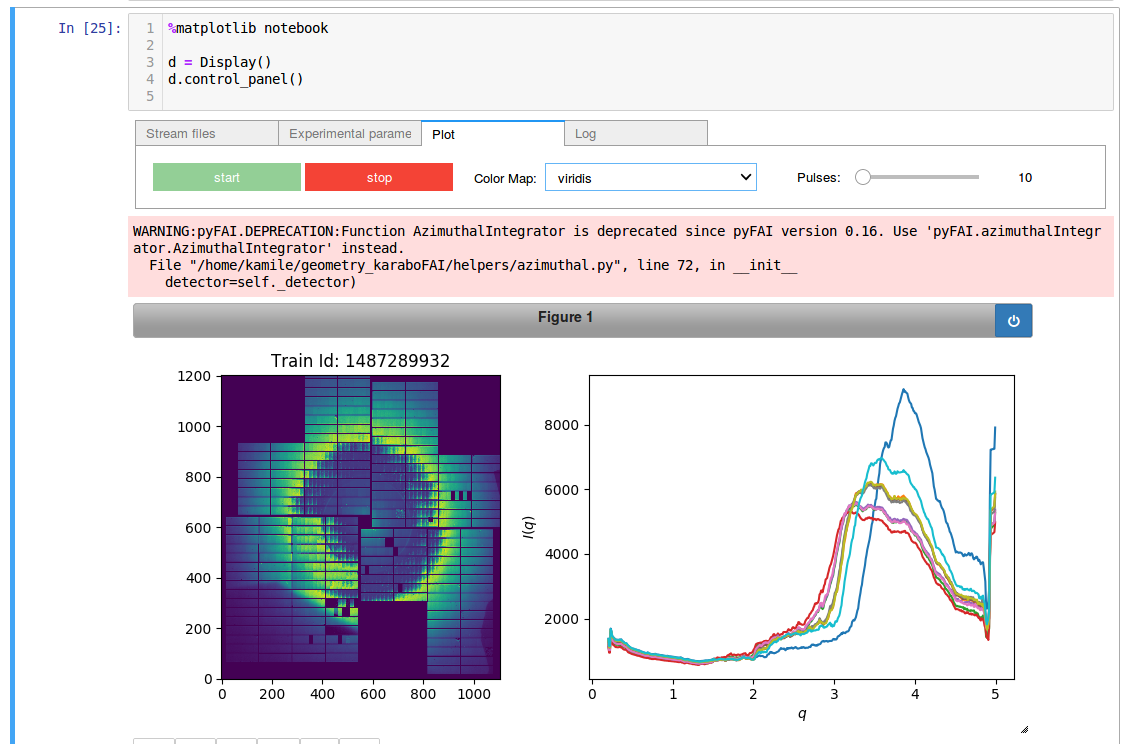
\includegraphics[height=0.27\textheight]{images/photon-science-prototype2.png}
    \caption{Prototypes for data analysis of 2d x-ray detector images
      in the Jupyter notebook, relating to the
      photon science use case.
      % task reference in caption doesn't work
      % \taskref{applications}{reproducibility-xfel}.
      \emph{(Left)} Data from crystallography
      scattering experiment. \emph{(Right)} Azimuthal integration of detector
      data as one step in the data analysis workflow.}
    \label{fig:photon-science-example}
  \end{figure}


  \emph{Context}: The very first experiments at European XFEL
  produced as little as 45 terabytes of data on average, but as the
  facility develops, the amount of data produced per time is expected
  to grow substantially: Given the rate of light pulses, there is the
  potential to produce up to a petabyte of data within the beam time
  of one experiment (typically one week). These significant amounts of
  data need to be complemented by complicated workflows to convert the
  data into insight through data analysis. Derived results of such
  data analysis are typically much smaller in size and useful to
  archive together with the raw data. To explain how they have been
  obtained, the particular workflow of data analysis also needs to be
  archived.

  \medskip
  \emph{Vision}:
  At European XFEL, it is proposed to use Jupyter notebooks to facilitate
  this workflow: the simplest model would be to use one notebook per
  workflow. Once the data capture from the experiment is completed,
  this notebook can be executed (without being displayed in a web
  browser) to start processing the data. When the notebook has
  completed execution, it is saved, and contains the analysis results
  (it may of course also created files on disk as part of the
  process).

  A particularly useful aspect of the notebooks is that they mix data
  analysis commands with outputs, and that the notebook provides a
  complete (and thus reproducible) summary of the data analysis when
  it succeeds with the execution. Should the execution fail, for
  example half-way through the notebook, then derived results obtained
  prior to the error occurring are preserved and can be inspected. The
  error is embedded in the notebook and appears after the command that
  has triggered the error; which helps with debugging the process.

  This is of particular interest as the data analysis processes at
  European XFEL may fail not because of software errors but due to
  variation in the data that require (manual) expert adjustments of
  parameters. The ``failure'' of such an analysis workflow
  (represented through the Notebook) is thus not exceptional, but a
  common occurrence. The scientist conducting the experiment is
  sufficiently skilled to modify the parameters and wants to either
  re-execute the notebook from the beginning or to continue from the
  point of failure. The notebook caters for both use cases. The
  modified notebook would need to be preserved of course to provide
  reproducibility of the derived results that the notebook has
  computed.

  We are aiming for re-executability of the notebook for the lifetime
  of the data. The lifetime of the archived data at European XFEL is
  currently guaranteed for 5 years and aimed to be 10 years
  \cite{EuXFEL-datapolicy-2017}. It is possible though, that data used
  for publications will be preserved for longer, and it would be
  highly desirable to keep the data analysis re-executable for the
  same period of time, potentially well exceeding 10 years.

  The particular activities for this demonstrator are shown in
  \WPref{applications} in \taskref{applications}{reproducibility-xfel}.
